% acmlarge-sample.tex, dated 25th May 2012
% This is a sample file for ACM large trim journals
%
% Compilation using 'acmlarge.cls' - version 1.3, Aptara Inc.
% (c) 2011 Association for Computing Machinery (ACM)
%
% Questions/Suggestions/Feedback should be addressed to => "acmtexsupport@aptaracorp.com".
% Users can also go through the FAQs available on the journal's submission webpage.
%
% Steps to compile: latex, bibtex, latex latex
%
% For tracking purposes => this is v1.3 - May 2012

\documentclass[prodmode,acmtomccap]{acmlarge}
\usepackage{tikz,relsize,microtype,lipsum,csquotes,
	enumerate,amssymb,fixltx2e,blindtext,amsmath,mathtools }
\usepackage{graphicx}
\graphicspath{{img/}}

\blindmathtrue


% Metadata Information
\acmVolume{1}
\acmNumber{1}
\acmArticle{1}
\articleSeq{1}
\acmYear{2012}
\acmMonth{7}

% Package to generate and customize Algorithm as per ACM style
\usepackage[ruled]{algorithm2e}
\SetAlFnt{\algofont}
\SetAlCapFnt{\algofont}
\SetAlCapNameFnt{\algofont}
\SetAlCapHSkip{0pt}
\IncMargin{-\parindent}
\renewcommand{\algorithmcfname}{ALGORITHM}

\providecommand{\abs}[1]{\lvert#1\rvert}


% Page heads
\markboth{Daniel Watzinger}{Multi-Provider Virtual Network Provisioning}

% Title portion
\title{Multi-Provider Virtual Network Provisioning}
\author{DANIEL WATZINGER\affil{University of Passau}}

\begin{abstract}
Network virtualization is widely regarded as the next big step to facilitate a new polymorphic future Internet, which enables sharing of physical substrate resources, 
efficient resource utilization and coexistence of heterogeneous network architectures. Previous research has concentrated on Service Providers acquiring resources
from a single Infrastructure Provider. This paper analyzes two different approaches to tackle virtual network provisioning in a multi Infrastructure Provider environment.
The former focuses on technical aspects of the provisioning process and introduces a new actor called Virtual Network Provider  to the existing business model.
Provisioning is classified into several steps and detailed algorithmic solutions are given for each. Splitting of the request topology across different substrate networks
is solved by both a reduction to a max-flow/min-cut problem and linear program formulation. Embedding of resulting segments is resolved by a mixed integer program formulation that
simultaneously embeds nodes and links as well as provides parallel processing capabilities.
The latter proposes a Vickrey-based auction model called V-Mart that provides a complete framework for the provisioning process. V-Mart enables Service Providers to minimize
their costs and offers an environment where Infrastructure Providers are able to compete in a faithful and market-driven manner.
Both proposals are evaluated through simulation in terms of performance. In addition, thoughts on energy efficiency are given.
\end{abstract}

\category{C.2.1}{Computer Systems Organization}{Computer-Communication Networks}[Network Architecture and Design]

\terms{Algorithms, Design, Economics, Theory}
\keywords{Network Virtualization, Future Internet, Virtual Network Provisioning, Multi-Provider Request Splitting and Embedding, Fair Market Provisioning, Energy Efficiency}

%\acmformat{Pineo, D. and Ware,  C. 2010.Neural Modeling of Flow Rendering Effectiveness.}

\begin{document}

%\begin{bottomstuff}
%This work originated from an advanced seminar on "Energy efficient virtual networks" at the University of Passau.\\
%Author's address: Daniel Watzinger; email: daniel.watzinger@gmail.com
%\end{bottomstuff}
\maketitle

% Introduction
\section{Introduction}
\label{sec:introduction}

\small

Network virtualization is one of the keys to a new polymorphic future Internet. Its basic entity is called a 
\emph{virtual network~(VN)} that is composed of \emph{virtual nodes} and \emph{virtual links}. It can be described as
a logical overlay on top of the physical topology.
During the \emph{virtual network provisioning} work-flow the main task is to determine a mapping 
-- called \emph{embedding} -- of \emph{virtual nodes} to physical ones as well as of virtual links to physical links or paths.
The underlying physical network is commonly referred to as \emph{substrate network}.
After \emph{provisioning}, the synthesized \emph{virtual network} resembles a traditional physical network.

This leads to both great flexibility and abstraction from physical aspects of the network. Network protocols may be exchanged easily. 
\emph{Virtual networks} can be deployed and torn down on-demand, 
\emph{on-line} and on top of each other thus leading to sharing and efficient utilization of physical resources, which in turn boosts energy efficiency, 
as well as coexistence of heterogeneous network architectures.

The traditional role of \emph{Internet Service Providers~(ISPs)} is subdivided into two new actors within the \emph{Network Virtualization Environment~(NVE)} denoted by 
\emph{Infrastructure Providers~(InPs)} and \emph{Service Providers~(SPs)} respectively.
\emph{Infrastructure Providers} are in charge of managing the substrate network and its physical resources. Furthermore, they are responsible for partitioning the physical resources
into virtual ones and to provide programmable interfaces to administrate these virtual entities.
\emph{Service Providers} are customers to \emph{InPs} and lease virtual resources to realize their desired \emph{virtual networks}, which in turn provide services to \emph{end users}.

\emph{SP}-to-\emph{InP} customer relationships are called \emph{vertical relations}. Note that both actors may switch roles in the event of an 
\emph{SP} re-offering its acquired resources or \emph{InPs} purchasing from one another.
 In the case of a multi-provider environment, meaning an environment where two or more
\emph{InPs} can host at least parts of the desired \emph{VN}, a \emph{SP} is likely to try to minimize its costs by splitting the \emph{VN} topology across multiple substrate networks.
Hosting of large \emph{VNs} that cannot be allocated by one individual \emph{InP} exclusively by a collective effort of several providers is another reason for a \emph{SP}
to subdivide its topology into segments.
Links connecting two disjoint substrate networks of different \emph{InPs} are called \emph{inter-domain} links in opposition to 
\emph{intra-domain} links within substrate bounds. Such a \emph{InP-to-InP} relationship is referred to as \emph{horizontal}. 
Splitting of the virtual network topology may occur in a \emph{private} manner where all participating \emph{InPs} peer
to provide a packaged deal to the \emph{SP}. However, much more desirable is a \emph{public} splitting process, where the partitioning of the topology originates from a customer- and
market-driven environment.

The remainder of this paper analyzes two different approaches to tackle the \emph{virtual network provisioning} with a focus on multi-provider environments.
In \citeN{Houidi}, the authors classify the \emph{provisioning} process into several disjoint steps and provide detailed algorithmic solutions for each.
In addition, they introduce an new actor called \emph{Virtual Network Provider} to the existing business model. Changes to the business model as well as
classification of the \emph{provisioning} are discussed in section~\ref{sec:provisioning}.
In section~\ref{sec:splitting}, splitting of the request topology across different substrate networks is shown to be a NP-hard problem even for two participating \emph{InPs}. 
Additional but reasonable presumptions are made to solve the splitting by reduction to a \emph{max-flow/min-cut problem} in case of two providers.
The general case is solved by a recursive heuristic, which falls back on the network flow solution. Furthermore, a linear program formulation of the \emph{VN Splitting} problem
is given to evaluate the aforementioned heuristic.
Embedding of resulting segments is resolved by a mixed integer program formulation, which is able to simultaneously embed nodes and links and process embedding request in parallel.
Key ideas and evaluation results of this approach are given in section~\ref{sec:embedding}.

Section~\ref{sec:vmart} provides a different solution for the \emph{provisioning} process introduced by \citeN{Zaheer}.
This approach is loosely based on a \emph{Vickrey} auction model and focuses on economic aspects. It does not impose particular pricing models on the \emph{InPs} but facilitates
deployment of diverse pricing policies like \emph{volume discount} or \emph{package pricing}. Furthermore, a new concept denoted by \emph{co-location} is presented
to ensure performance guarantees in a multi-provider environment.

Thoughts on energy efficiency of both proposals are given in section~\ref{sec:efficiency}.


\section{Virtual Network Provisioning}
\label{sec:provisioning}
The authors of \citeN{Houidi} introduced a new actor called \emph{Virtual Network Provider~(VN~Provider)} -- known also as \emph{Connectivity Provider} -- 
to the \emph{Network Virtualization Environment} business model. The \emph{VN Provider} serves as a broker for both \emph{Service} and \emph{Infrastructure Providers}.
Its task is to abstract from the complexity of \emph{virtual network provisioning}, especially in the multi-provider case. \emph{SPs} commit their desired virtual network topologies
to the \emph{VN provider} which subsequently seeks and aggregates matching resources from suitable \emph{InPs} in order to synthesize \emph{VNs}.
Figure~\ref{fig2} visualizes the placement of this new actor in the resulting business model.

\begin{figure}[htb]
	\centering
	
\includegraphics[width=0.7\textwidth]{broker}
	\caption{A \emph{Virtual Network Provider} serves as a broker for  both \emph{Service} and \emph{Infrastructure Providers}}
	\label{fig2}
\end{figure}

\emph{VN provisioning} occurs in four main phases namely \emph{Resource Matching}, \emph{VN Request Splitting}, \emph{VN Embedding} and \emph{Resource Binding}.
Figure~\ref{fig3} depicts the work-flow of the \emph{provisioning} process.

\begin{figure}[htb]
	\centering
	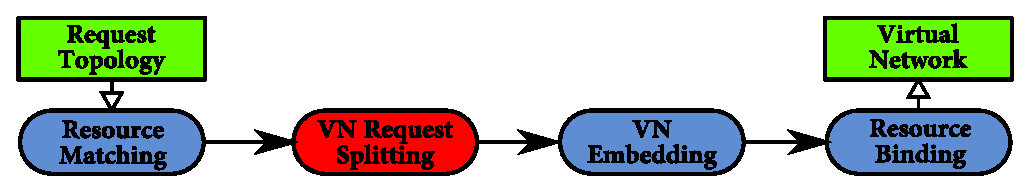
\includegraphics[width=0.7\textwidth]{provisioning2}
	\caption{The workflow of the \emph{provisioning} process. The most important \emph{VN Request Splitting} step is highlighted in red.}
	\label{fig3}
\end{figure}

\emph{Resource Matching} tries to determine a set of matching substrate nodes for each \emph{virtual node}.
To gather the required data for the  \emph{Resource Matching} step, \emph{InPs} that want to offer their available resources must publish information about these resources
to a \emph{Resource~Discovery~Framework~(RDF)}. Data about substrate resources is divided into two disjoint sets

\begin{describe}{{\bfseries Non-Functional attributes\/}:}
	\item[\bfseries Functional attributes:] Define static characteristics and properties of substrate resources up to and including node type, node capacity, link type, geolocation and costs.
	\item[\bfseries Non-Functional attributes:] Composed of dynamic or real-time parameters like available node and link capacity or \emph{Quality of Service} constraints.
\end{describe}

Only \emph{functional attributes} are published to the \emph{RDF} by \emph{InPs} since dynamic characteristics are prone to frequent updates and more importantly
are often desired to remain proprietary knowledge to \emph{InPs}. Subsequently, the \emph{Resource~Discovery~Framework} is responsible for structuring the received data
using \emph{dendrograms}, which are a type of binary trees. \emph{Dendrograms} are the result of agglomerative clustering techniques. In this case, \emph{conceptual clustering}
is used to organize and group resources with similar concepts, descriptions and properties into clusters, thus producing a hierarchy of conceptual clusters (see figure~\ref{fig4}).


\begin{figure}[htb]
	\centering
	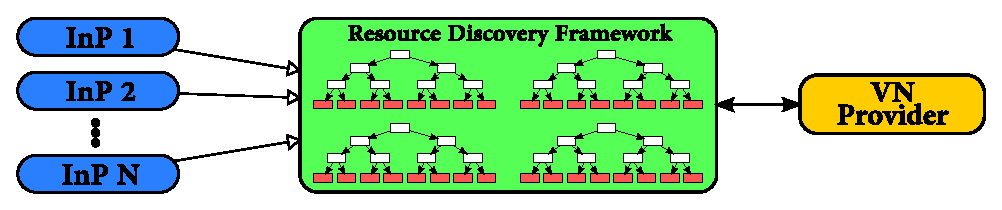
\includegraphics[width=0.7\textwidth]{rdf}
	\caption{\emph{InPs} advertise available resources with the help of a discovery framework. 
		Subsequently,  the \emph{Virtual Network Provider} uses the \emph{Resource~Discovery~Framework} to determine a set of matching substrate nodes for each \emph{virtual node}}
	\label{fig4}
\end{figure}

Based on the previous step, the \emph{VN provider} makes use of a similarity based matching algorithm to determine the most similar clusters for each \emph{virtual node}, thereby associating a set of matching substrate
nodes with each \emph{virtual node}. Note that the resulting sets of matching substrate nodes may contain nodes from different \emph{InPs} within a multi-provider environment.

\section{Virtual Network Splitting}
\label{sec:splitting}
As noted above, the \emph{Resource Matching} phase yields a mapping from each \emph{virtual node} to a set of substrate nodes capable of hosting it, which may additionally belong to different \emph{InPs}.
The request topology is represented using an undirected graph. 
The next step conducted by the \emph{VN Provider} is to efficiently partition the request topology in order to minimize the provisioning costs of the \emph{SP} and to implement large \emph{virtual networks}
that cannot be hosted by one \emph{InP} exclusively. In other words, the request topology is subdivided into segments that should be hosted by different \emph{InPs} in such a way as to
minimize the total costs for provisioning the \emph{VN}.

Two different scenarios are discussed in \citeN{Houidi}. Firstly, the case with only two \emph{Infrastructure Providers} is analyzed. Afterwards, the general case with more than two \emph{InPs} involved
is examined. The authors assume that the following costs for each substrate node and possible links are known to the \emph{VN provider} beforehand

\begin{describe}{{\bfseries Inter-domain costs\/}:}
	\item[\bfseries Node costs:] $C_i^X$ denotes the costs of hosting \emph{virtual node} $i$ by \emph{Infrastructure Provider} $X$ 
	\item[\bfseries Intra-domain costs:] $C_{ij}^X$ represents the costs of provisioning a link between \emph{virtual nodes} $i$ and $j$ within the substrate of \emph{InP} $X$ 
	\item[\bfseries Inter-domain costs:] $C_{ij}^{XY}$ denotes the costs of provisioning a link between \emph{virtual nodes} $i$ and $j$ across substrate bounds involving \emph{InP} $X$ and \emph{InP} $Y$ respectively	
\end{describe}

\subsection{Splitting across two Infrastructure Providers}
Consider a variable $x_i$ for each \emph{virtual node} $i$ that either equals $1$ or $0$ if $i$ is allocated by the first or second \emph{InP}. Finding the optimal cost-minimizing solution for
\emph{VN Splitting} can then be modeled by a simple \emph{0-1 quadratic program} formulation

\normalsize

\[
 \phi
   \begin{dcases}
		\min \sum\limits_{i} \underbrace{x_i C_i^1 + (1-x_i) C_i^2 }_{\text{node costs}}
			+ \sum\limits_{i < j} \underbrace{x_i x_j C_{ij}^{1} + (1 - x_i)(1 - x_j) C_{ij}^{2}}_{\text{possible intra-domain links}}
			+ \underbrace{x_i (1 - x_j) C_{ij}^{12} + (1 - x_i)x_j C_{ij}^{21}}_{\text{possible inter-domain links}} \\
		\forall i : x_i \in \{ 0,1\}
   \end{dcases}
\]

\small

It remains to show that \emph{VN Splitting} is in fact a NP-hard problem. The authors use a reduction from \emph{MAX-2-SAT} $\in~NP$. \mbox{\emph{MAX-2-SAT}} instances
are Boolean formulas in \emph{conjunctive normal form}
featuring exactly two literals per clause. The goal of \mbox{\emph{MAX-2-SAT}} is to find a fitting assignment of Boolean variables in order to maximize the number of satisfied clauses. Consider an arbitrary 
\mbox{\emph{MAX-2-SAT}} problem instance with Boolean variables $y_k$

\normalsize

$$
(y_a \vee y_b) \wedge (y_c \vee y_d) \wedge \dots \wedge (y_i \vee y_j)
$$

\small

Finding an assignment that minimizes the number of clauses that are not satisfied is equivalent to maximizing the number of those that are satisfied. This duality helps to reduce the complexity of the problem
since it is clear that $(y_i \vee y_j)$ is false if and only if both variables equal false or correspondingly $(\lnot y_i \wedge \lnot y_j)$ is true.
Building a \emph{VN Splitting} instance is done by considering a \emph{virtual node} $i$ for each Boolean variable $y_i$. Additionally, all provisioning costs equal zero, particularly node hosting costs $C_i^{X}$,
with the exception of the following rules

\normalsize

$$
\begin{array}{cccccccccccccccc}
	(y_i \vee y_j) & \Rightarrow & C_{ij}^2 = 1 &;& (\lnot y_i \vee y_j) & \Rightarrow &C_{ij}^{12} = 1 &;& (y_i \vee \lnot y_j) & \Rightarrow & C_{ij}^{21} = 1 &;& (\lnot y_i \vee \lnot y_j) & \Rightarrow & C_{ij}^1 = 1
	
\end{array}
$$

\small

A solution for the original \emph{MAX-2-SAT} problem is then obtained by solving the resulting \emph{VN Splitting} instance, using costs as defined above. If the first \emph{InP} allocates node $i$
then $z_i$ is assigned $true$, analogously $z_i$ equals $false$ if the second \emph{InP} hosts the corresponding \emph{virtual node}. In addition, by construction the minimum 
total provisioning costs equal the number of unsatisfied clauses.
The reduction can clearly be achieved in polynomial time. Thus it follows that \emph{VN Splitting} across two \emph{InPs} is NP-hard.

\subsection{Max-flow/Min-cut formulation}
However, by adding some reasonable constraints to the link costs, splitting can be achieved in polynomial time. By assuming that provisioning of an \emph{inter-domain} link is always more expensive
than setup of an \emph{intra-domain} link, the problem may be reduced to a network flow problem, which is subsequently solved using \emph{max-flow/min-cut} algorithms like \emph{Edmonds-Karp}
or \emph{Dinitz blocking flow}.

\normalsize

$$
	\forall i,j: C_{ij}^{12} \geq C_{ij}^1 \wedge C_{ij}^{21} \geq C_{ij}^2
$$

\small

To obtain a \emph{max-flow/min-cut} instance the original request topology is extended to a flow network, which is a directed weighted graph, by adding a source $s$ and a sink $t$.
Additionally, the following edges and their corresponding flow capacities are appended. Consider that $N(i)$ denotes the set of adjacent \emph{virtual nodes} to $i$.

\begin{enumerate}
	\item An edge from the source $s$ to every \emph{virtual node} $i$ with a weight equal to $C_i^2 + \sum\limits_{k < i, k \in N(i)} C_{ik}^2$
	\item An edge from every \emph{virtual node} $i$ to the sink $t$ with a flow capacity equal to $C_i^1 + \sum\limits_{k < i, k \in N(i)} C_{ik}^1$
	\item Ultimately, for each undirected edge $e=\{i,j\}$ belonging to the original request topology two directed edges are added. Without loss of generality it is assumed that $j < i$.
		Both, an edge from $i$ to $j$ featuring a capacity of $C_{ij}^{12} - C_{ij}^1$ and its back-edge from $j$ to $i$ with a weight equal to $C_{ij}^{21} - C_{ij}^2$ are appended.
\end{enumerate}

\begin{figure}[htb]
	\centering
	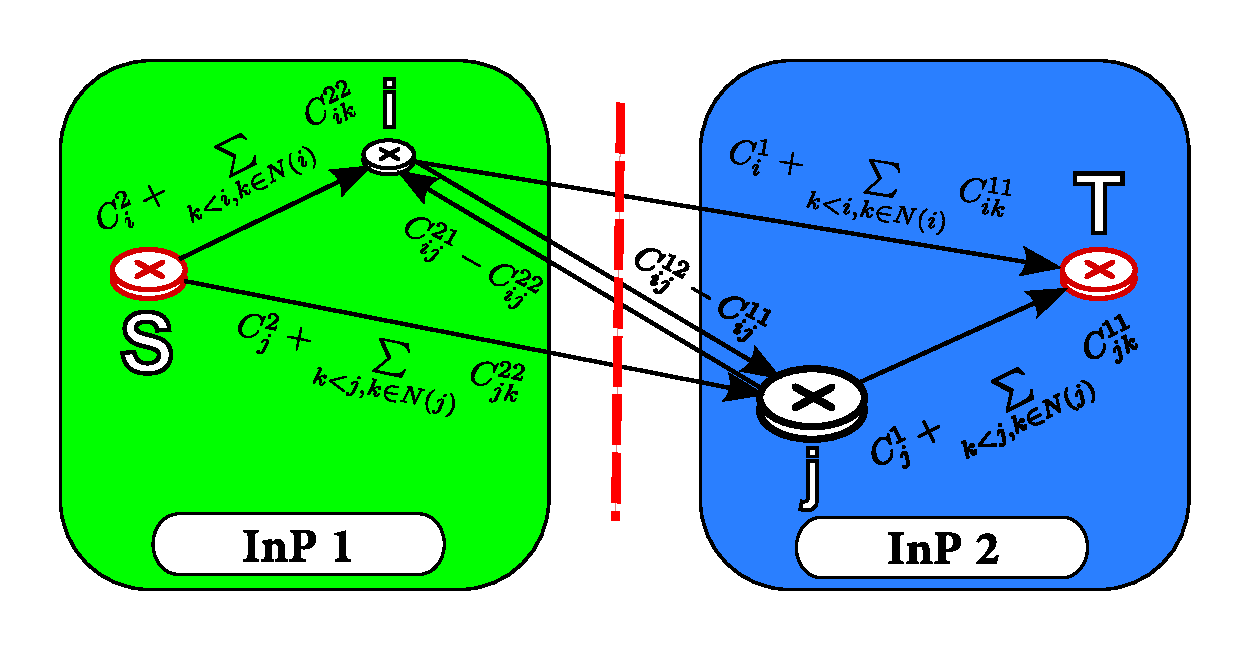
\includegraphics[width=0.6\textwidth]{maxflow}
	\caption{Expansion of a request topology to a flow network with corresponding edge capacities. Note that $j < i$ holds in this example.}
	\label{fig5}
\end{figure}

A minimal example of extending a request topology, consisting of two \emph{virtual nodes} $i$ and $j$ connected by a link, is visualized in figure~\ref{fig5}.
Due to the aforementioned constraints over link costs, each edge capacity in the resulting flow network equals a non-negative number at all times. This is an important fact since
\emph{max-flow/min-cut} instances with negative capacities are known to be NP-hard using a simple reduction from \emph{MAX-CUT}.
Subsequently, the \emph{max-flow/min-cut} problem is solved using well known algorithms that run in polynomial time. The solution provides a partitioning of the network and its nodes
into two disjunctive subsets. An optimal solution for the original \emph{VN Splitting} instance is obtained by allocating \emph{virtual nodes} enclosed within the subset containing the source by the first \emph{InP}.
\emph{Virtual nodes} belonging to the subset that contains the sink are provisioned by the second \emph{InP}.

Furthermore, the size of the \emph{min-cut} equals the total and minimal
costs to provision the \emph{VN}. Consider two subsets $S$ and $T$ denoting the partitioning obtained by a \emph{max-flow/min-cut} solution containing $s$ and $t$, respectively.
It follows, that the size of any cut (the capacity of cut edges from $S$ to $T$), particularly the size of the \emph{min-cut}, is given by

\normalsize

$$
	\underbrace{\sum\limits_{i \in S} C_i^1 + \sum\limits_{i \in T} C_i^2}_{\text{node costs}} + 
	\underbrace{\sum\limits_{i,j \in T, i < j, j \in N(i)} C_{ij}^2 + \sum\limits_{i,j \in S, i < j, j \in N(i)} C_{ij}^1}_{\text{intra-domain costs}}
	+\underbrace{\sum\limits_{i \in S, j \in T, j \in N(i)} C_{ij}^{12}}_{\text{inter-domain costs}}
$$

\small

Therefore, by minimizing the cut size the provisioning costs are minimized. Thus  solving the network flow problem yields an optimal solution for \emph{VN Splitting} across two \emph{InPs}.

\subsection{Splitting across multiple Infrastructure Providers}
If more than two \emph{InPs} are able to host at least some parts of the desired \emph{virtual network}, \emph{VN Splitting} stays NP-hard even if the assumptions introduced in the previous section are met.
The authors of \citeN{Houidi} provide a proof by reduction from the \emph{3-MULTIWAY-CUT} problem and provide a heuristic to recursively solve the problem by falling back to methods developed
for the \emph{two-provider case}.

Firstly, a preprocessing step that clusters \emph{InPs} based on their cost similarities is executed. The clustering algorithm operates in an agglomerative manner by recursively merging two
\emph{InPs} that are the most similar, yet again yielding a dendrogram. This time leafs of the dendrogram represent actual \emph{InPs}
whereas inner nodes are formed by \emph{logical InPs}. Consider two \emph{InPs} $X$ and $Y$, the dissimilarity metric $d$ is given by

\normalsize

$$
 d(X,Y) = \sqrt{\sum\limits_{i} \abs{C_i^X - C_i^Y}^2 + \sum\limits_{i, j \in N(i)} \abs{C_{ij}^X - C_{ij}^Y}^2}
$$

\small

During each iteration, two \emph{InPs} $X$ and $Y$ are merged into one \emph{logical InP} $L$. Its costs are approximated based on the costs of the grouped \emph{InPs} as follows

\normalsize

$$
\begin{array}{cccc}
	C_i^L = \frac{C_i^X + C_i^Y}{2} & C_{ij}^{L} = \frac{C_{ij}^{XY} + C_{ij}^{YX} + C_{ij}^{X} + C_{ij}^{Y} }{4} & 
	C_{ij}^{LZ} = \frac{C_{ij}^{XZ} + C_{ij}^{YZ}}{2} & C_{ij}^{ZL} = \frac{C_{ij}^{ZX} + C_{ij}^{ZY}}{2} 
\end{array}
$$

\small

Secondly, the optimal \emph{max-flow/min-cut} solution is recursively applied at each plane of the dendrogram
since exactly two (possibly \emph{logical}) \emph{InP} and their corresponding costs are distinguished at each level of the binary tree. Thus one obtains a partitioning of the request topology.
Figure~\ref{fig6} depicts the process in an environment involving four \emph{Infrastructure Providers}. 

\begin{figure}[htb]
	\centering
	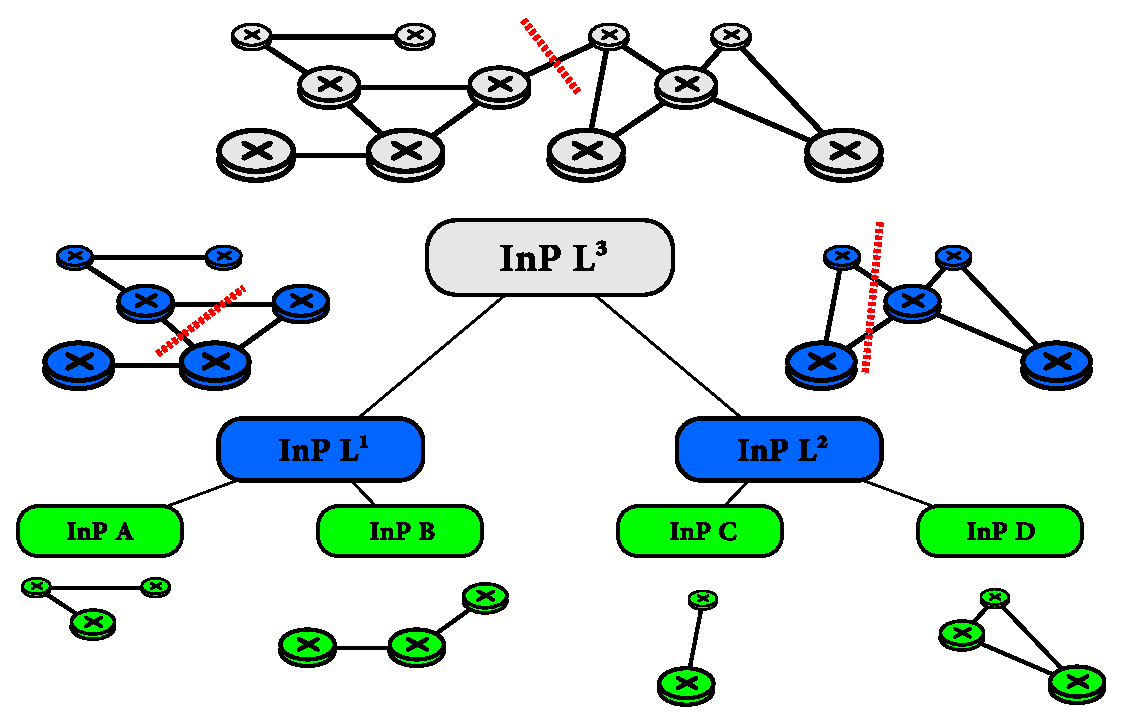
\includegraphics[width=0.6\textwidth]{recursive_heuristic}
	\caption{The heuristic \emph{max-flow/min-cut} solution across multiple providers splits the request topology recursively at each level of a binary tree, which is obtained 
		by agglomerative clustering of involved \emph{InPs} based on cost similarity}
	\label{fig6}
\end{figure}

\subsection{Evaluation}
The authors evaluate the performance of the \emph{max-flow/min-cut} algorithm and the heuristic introduced in the previous section
by simulation using \emph{partial} and \emph{full mesh VN} request topologies. 
Performance of the approaches is measured in comparison to an \emph{integer linear program (ILP)}, which provides an optimal solution for the general multiple \emph{InPs} scenario.
The \emph{ILP} is resolved using \emph{branch and bound} techniques. \emph{Max-flow/Min-cut} problems are solved using the \emph{Ford-Fulkerson} algorithm.

In the \emph{two-provider} case, solving the \emph{ILP} is slightly faster than obtaining a solution using the \emph{max-flow/min-cut} formulation up to a number of
50 \emph{virtual nodes}. Beyond this turning point, the network flow method shows to be much faster and scalable.

To evaluate the general multi-provider case, a scenario involving 5 \emph{InPs} is deployed. This time the turning point where the heuristic shows to be much more efficient than solving the \emph{ILP}
lies at approximately 30 \emph{virtual nodes} that form a \emph{partial mesh} topology whereas for \emph{full mesh} topologies the \emph{ILP} solution performs even worse.
As expected, the computing time for the \emph{ILP} increases exponentially with the size of the request topology.

In addition, extra costs caused by the heuristic solution are analyzed. Empirical tests show, that the extra costs are approximately upper-bounded by 2\% regarding a five \emph{Infrastructure Provider} case and
converge around 5\% with 10 \emph{InPs} involved.

\section{Virtual Network Embedding}
\label{sec:embedding}
After successful partitioning of the request topology, each involved \emph{InP} must try to embed the associated segment on its substrate.
The goal of embedding is to find an optimal mapping of each \emph{virtual node} onto a matching substrate node and to select an appropriate substrate path for every \emph{virtual link}.
This problem is known to be NP-hard. Former research into this subject proposed heuristic algorithms or near optimal solutions using linear programming techniques with
relaxed constraints. Most of the time these approaches treated embedding of nodes and links as separate phases.

The authors of \citeN{Houidi} propose an optimal solution of the problem with the help of a \emph{mixed integer program (MIP)} that tries to embed nodes and links simultaneously. In addition,
it features \emph{parallel request processing (PRP)}, that means embedding requests that arrive within a specific time-frame may be processed in parallel. Moreover,
\emph{sequential request processing (SRP)} is still available.
The \emph{MIP} is based upon a network flow formulation of the embedding problem.

\subsection{Evaluation}
Again, the embedding approach is evaluated by means of simulation of requests and substrate networks. The authors state, that there exists no known optimal embedding algorithm. Therefore, performance of the proposal
is measured against existing heuristics. Three key observations are made

\begin{enumerate}
	\item \emph{PRP} shows to lead to lower embedding costs compared to sequential processing due to more efficient usage of substrate resources.
	\item  The approach achieves higher acceptance ratios among \emph{InPs} since it provides an optimal solution with simultaneous embedding of nodes and links
		compared to heuristic approximations and near optimal solutions with relaxed constraints.
	\item Computing time of both \emph{PRP} and \emph{SRP} increases exponentially, thus the approach is only feasible for relatively small scale networks without dynamic environments.
		To exemplify, parallel processing of 4 embedding requests consisting of topologies with 6 \emph{virtual nodes} on a substrate of 30 nodes entails a delay of approximately 100 seconds
		compared to a few seconds using a heuristic.
\end{enumerate}

The last step of \emph{VN Provisioning} is denoted by \emph{Resource Binding} and deals with \emph{InPs} actually allocating and reserving the required substrate resources \emph{on-line} to synthesize
the desired \emph{VN}.

\section{V-Mart}
\label{sec:vmart}
To provide a fair market environment where \emph{SPs} are able to minimize their hosting costs for \emph{VNs} and \emph{InPs} can compete in a faithful and fair manner,
the splitting of \emph{VN} must be a \emph{public}, customer-driven process, in opposition to a \emph{packaged deal} negotiated in \emph{private} by the \emph{InPs}.
The proposal discussed in the previous sections qualifies as such a \emph{public} process. However, it does not deal with heterogeneous pricing models of involved \emph{InPs} since
the \emph{Resource~Discovery~Framework} solely advertises per-resource costs.

In \citeN{Zaheer}, a different approach to the \emph{provisioning} problem is discussed. \emph{V-Mart} concentrates on economic issues of the 
process and provides a complete framework for \emph{VN provisioning}.
The framework uses a two-stage \emph{Vickrey} auction model to deal with a multi-provider environment and the diverse pricing models of \emph{InPs} like 
\emph{volume discount} and \emph{packaged pricing}. In a \emph{Vickrey} auction, every bidder will quote a price for allocating a specific virtual resource. As is usually the case, 
the bidder with the best/lowest quote wins the auction, but will deliver the service at the price of the second lowest quote. \emph{Vickrey-based} auction models are known to be \emph{strategy-proof},
meaning that there exists only one dominating strategy for each bidder that is to quote a price proportional to the actual costs of rendering the service.

\emph{Provisioning} is mostly automated to support the \emph{on-demand} nature of the \emph{NVE}. Furthermore, it
efficiently solves splitting of the request topology using a local improvement heuristic.

\begin{figure}[htb]
	\centering
	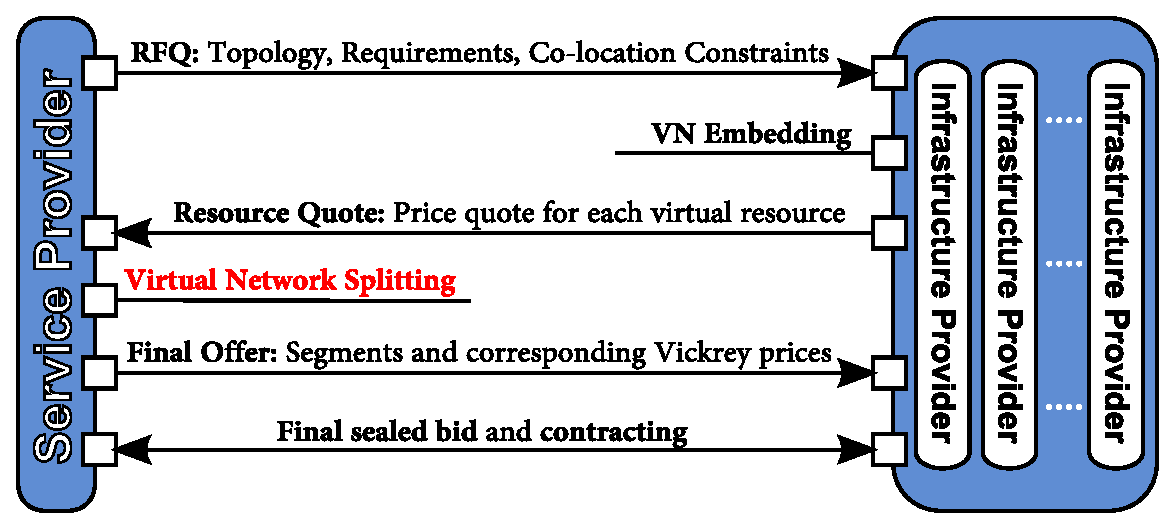
\includegraphics[width=0.7\textwidth]{vmart}
	\caption{The \emph{V-Mart} work-flow using a two stage \emph{Vickrey} auction model to provision a \emph{VN} in a multi-provider environment in a market-driven manner}
	\label{fig7}
\end{figure}

Figure~\ref{fig7} visualizes the \emph{V-Mart} work-flow. The process is composed of five main phases. 
Firstly, the \emph{SP} issues a \emph{Request for Quotation} including the desired request
topology, possible requirements concerning the virtual resources and a \emph{co-location} constraint to all \emph{InPs} taking part in the auction. In the following, \emph{InPs} involved in the auction
are often referred to as \emph{VN bidders}.

\emph{Co-location} is a new concept developed by the authors to overcome technical difficulties with
performance guarantees across substrate bounds. It is specified by an equivalence relation, which is reflexive, symmetric and transitive, over the set of \emph{virtual nodes}. The relation
states which \emph{virtual nodes} must be allocated by the same \emph{InP}. Thus  performance guarantees can be achieved for a group of resources. 
\emph{Co-location} is implemented by transforming the original request topology, represented by an undirected graph, into a \emph{V-Let meta-graph}. The \emph{meta-graph} is obtained
by combining nodes that belong to the same equivalence class to \emph{super-nodes} called \emph{V-Lets}. Each \emph{V-Let} is then regarded as an atomic entity that represents a set of nodes that must
be provisioned by the same \emph{InP}. Figure~\ref{fig8} depicts how a \emph{V-Let meta-graph} is obtained from the original request topology. Keep in mind that it is perfectly normal for a \emph{V-Let}
to consist of only a single \emph{virtual node}.

\begin{figure}[htb]
	\centering
	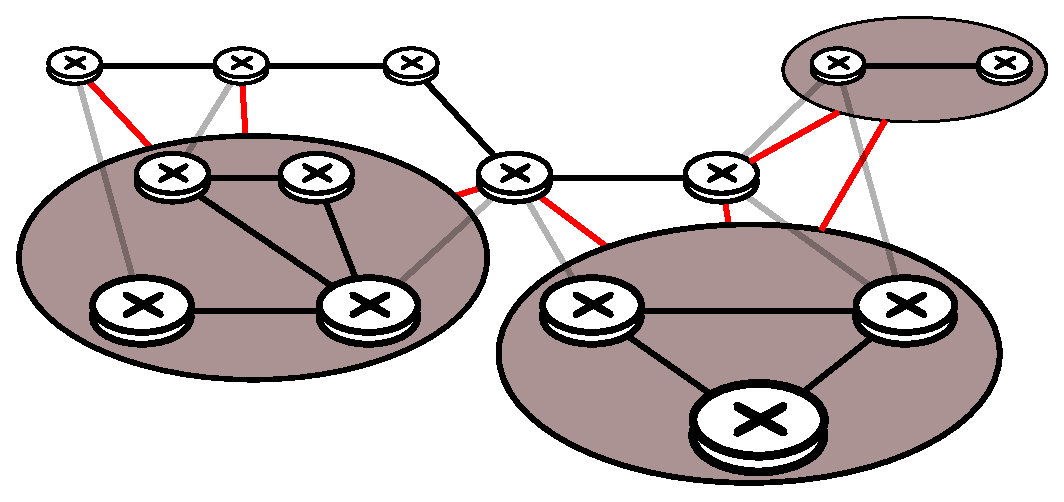
\includegraphics[width=0.6\textwidth]{colocation}
	\caption{A \emph{V-Let meta-graph} obtained from a traditional request topology by combining nodes belonging to the same equivalence class to \emph{V-Lets} (gray \emph{super-nodes}) based on the
		\emph{co-location} constraint}
	\label{fig8}
\end{figure}

In a second step, each \emph{VN bidder} tries to embed the whole \emph{VN} in order to determine the resources which it is able to host and to estimate its per-resource costs. Subsequently, 
the \emph{InPs} place a sealed resource quote under the \emph{Vickrey} model for each resource they are willing to host.

By the end of the last phase, the \emph{SP} has knowledge about price quotes for each virtual resource from possibly different \emph{VN bidders}. The \emph{SP} now modifies every
resource quote of each bidder to its \emph{Vickrey} quote, meaning the next best quote in sequence. Consider virtual resource $R$ and associated price quotes $a \leq b \leq c$ from three \emph{VN bidders}.
Then the \emph{Vickrey} quote for $a$ is $b$, $b$ is modified to $c$ and $c$ is left unchanged.
Using these modified resource quotes, the \emph{SP} partitions the \emph{V-Let meta-graph} into segments
in order to minimize total hosting costs by means of an iterative local improvement heuristic. The local improvement algorithm operates on an initial partition of the topology. Two different initial partitions are
examined by the authors, namely

\begin{describe}{{\bfseries Min-Cost\/}}
	\item[\bfseries Min-Cost] which assigns each \emph{V-Let} greedily to the bidder with the best quote under the \emph{Vickrey} auction model.
	\item[\bfseries Min-Cut] which tries to greedily assign non-overlapping subgraphs to the same \emph{InP} in descending order of subgraph size. Total quoted resource costs are used as a \emph{tie-breaker}
		in case of equal subgraph size. Eventually it is not feasible to form another subgraph. The remaining \emph{V-Lets} are then assigned according to the aforementioned \emph{Min-Cost} paradigm.
\end{describe}

Since both initial partitions neglect link costs and in particular \emph{inter-domain} link costs, local improvement iterations are made to further reduce the overall provisioning costs by moving
\emph{V-Lets} between partitions. In each iteration, a particular \emph{V-Let} $v$ is moved from \emph{InP} $X$ to $Y$ if it produces a positive gain based on the following metric

$$
	g_{X,Y}(v) = \beta \cdot (\text{decrease in link costs}) - \alpha \cdot (\text{increase in V-Let costs}) = -\left(\beta \cdot (\Delta \text{ link costs}) + \alpha \cdot (\Delta \text{ V-Let costs})\right) 
$$

In other words, a \emph{V-Let} is moved to another partition if the resulting linear weighted decrease in link provisioning costs is greater than the increase in V-Let hosting costs.
Local improvement terminates if a maximum of $k$ iterations is reached or if the current iteration does not produce a single positive gain.

In a penultimate step denoted by \emph{Final Offer}, the \emph{SP} sends the obtained segments along with the corresponding winner and \emph{Vickrey-Price} for each segment to all \emph{VN bidders}.
Each \emph{InP} may now place a final sealed quote, upper-bounded by the winning \emph{Vickrey-Price}, for every segment it wants to host.

The \emph{SP} contracts each segment to the bidder with the lowest quote according to the final auction round. If the final quote for a particular segment equals the \emph{Vickrey} winning price, it is contracted to
the winning \emph{VN bidder} of the first \emph{Vickrey} round.

\subsection{Pricing models}
The first sealed \emph{Vickrey} auction round is needed by the \emph{SP} to obtain a fair-market cost estimation for its \emph{VN provisioning} costs. 
Based on this estimation, the \emph{SP} is able to minimize its costs by partitioning the request topology.
The second and final auction round supports the diverse pricing models of \emph{InPs}.

Consider a \emph{VN bidder} with a \emph{volume discount} strategy. During the first \emph{Vickrey} round it places its per-resource quotes at non-discounted rates.
Discounted prices are then quoted in the final round since the exact resource count for each segment is no longer subject to change.

On the other hand, \emph{V-Mart} supports \emph{packaged pricing} models where a seller wishes to sell a specific package of resources at a discounted price.
In the first round, the \emph{VN bidder} may place per-resource quotes at non-reduced rates. However, following this strategy the bidder risks that the \emph{SP}
will segment its original package quote. To avoid a mismatch of the partitioning of the \emph{VN} and the original package, the dominating strategy for the \emph{InP}
is to place discounted per-resource quotes, computed based on the package price, during the \emph{Vickrey} auction round. Thus it is more likely that the package is preserved
whilst partitioning. In addition, the framework may be tuned to serve a market environment that adopts \emph{packaged pricing} by
setting a low $\frac{\beta}{\alpha}$ ratio within the gain metric. A low ratio favors increase in node costs over decrease in link costs and helps to preserve the original package unless there
exists another \emph{VN bidder} featuring far lower prices for a majority of the same resources.

\subsection{Evaluation}
The authors of \citeN{Zaheer} evaluated their proposal by simulation. Two main observations are made

\begin{enumerate}
	\item The internal ratio $\frac{\beta}{\alpha}$ should be set according to the pricing model mix within the market. A high ratio favors \emph{resource-wise}
		pricing strategies whereas the opposite is true for \emph{packaged pricing} models. The turning point approximately lies around $\frac{\beta}{\alpha} = 1$.
	\item The probability of an \emph{InP} being able or willing to host a particular resource determines which initial partition paradigm performs best in terms of overall costs 
		during partitioning of the \emph{VN}. If the probability is high, meaning each \emph{VN} bidder is able to host most or even all resources, \emph{Min-Cut} obtains
		better results than \emph{Min-Cost}. The converse is true for a low provisioning probability where the \emph{Min-Cost} paradigm performs best.
\end{enumerate}

\section{Energy Efficiency}
\label{sec:efficiency}
Energy efficiency has become an important issue in design and application of computer networks and will gain even more importance in the future. 
Increased ecological awareness and ever rising energy costs justify this track.
Thus it is only reasonable to briefly analyze both aforementioned proposals in terms of energy efficiency.
 
Traditional network architectures are usually designed to cope with peak loads, which in turn leads to low capacity utilization under average load scenarios due to over-provisioning.
Network virtualization overcomes this deficiency by means of resource consolidation. Underutilized physical substrate resources may be dynamically switched off or hibernated and their services
assigned to other resources in times of low traffic demands.

Since energy consumption is considered a dynamic or \emph{non-functional} substrate attribute, it is not published to the \emph{Resource~Discovery~Framework}
by \emph{InPs}. Therefore, the \emph{VN Provider} is not aware of the current energy use and cannot partition the desired \emph{VN} topology across multiple
\emph{InPs} in an energy efficient manner. Furthermore, the dynamic and fluctuating nature of power consumption would require constant repartitioning and recontracting
of the \emph{VN} topology which is not desirable nor technically feasible in an \emph{on-line} way.

In addition, there exists another significant economic issue.
Consider that substrate resources of different \emph{InPs} obey a simple linear power consumption model. In linear models, the power consumption scales linear with the current workload up
to the maximum power consumption starting at an usually large constant. Therefore switching on of sleeping or hibernated resources is considered expensive.
An energy-aware \emph{VN Provider}, which is trying to partition a \emph{VN} request topology in an energy efficient manner, is likely
to assign segments to \emph{InPs} whose substrate resources are already partly utilized. Thus these established \emph{InPs} possess an unfair advantage over new 
providers with mostly idle substrate network parts. Such an environment is not fitting for market-driven competition of \emph{InPs}.

However, the \emph{VN Embedding} phase of both approaches is suited for consideration of energy consumption. Each involved \emph{InP} should try to embed
its subset of the \emph{VN} in an energy efficient way. \emph{Parallel request processing (PRP)}, introduced in section~\ref{sec:embedding}, seems especially
promising since it is able to embed several embedding request arriving within a particular time-frame in parallel, thus leading to optimal embedding in terms of costs and energy.
 
 
 \section{Conclusion}
\label{sec:conclusion}
This paper examined two different proposals for \emph{virtual network provisioning} with the focus on multi-provider environments.
The authors of \citeN{Houidi} provided a complete classification of the \emph{provisioning} process in several phases. 
In addition, detailed algorithmic solutions were given for each step. Transformation of the NP-hard \emph{VN Splitting} problem into 
a network flow formulation by assuming reasonable constraints over link costs is a major result. Furthermore, they provided the first
exact algorithm for \emph{VN Embedding} that is able to simultaneously embed links and nodes as well as process several embedding requests in parallel.

On the other hand, \emph{V-Mart}, introduced in \citeN{Zaheer}, tried to solve the \emph{provisioning} problem with the help of a \emph{Vickrey-based} auction system and 
focused on a customer- and market-driven environment.

Both approaches should be combined in order to eliminate certain deficiencies of both proposals. The concept of \emph{co-location} may be incorporated into the first approach
in order to achieve performance guarantees for particular subsets of the \emph{VN}.
Moreover, the \emph{max-flow/min-cut} formulation of the \emph{VN Splitting} problem is promising to replace the local improvement heuristic in \emph{V-Mart}.
Besides, \emph{VN Providers} should handle the  \emph{V-Mart} work-flow in order to decouple \emph{SPs} from the complexity of the auction system.


% Appendix
%\appendix
%\section*{APPENDIX}
%\setcounter{section}{1}


% Bibliography
\bibliographystyle{acmlarge}
\bibliography{doc}

% History dates
%\received{February 2009}{July 2009}{October 2009}


%\elecappendix


%\section{Analysis of Invalid Trials}
%\label{invalid}

\end{document}

